\documentclass[12pt]{article}
\usepackage[utf8]{inputenc}
\usepackage{amsmath, amssymb}
\usepackage{geometry}
\usepackage{enumitem}
\usepackage{fancyhdr}
\usepackage{booktabs}
\usepackage{longtable}
\usepackage{array}
\usepackage{multirow}
\usepackage{graphicx}
\usepackage{float}
\usepackage{caption}
\captionsetup{font=small}
\usepackage{hyperref}
\usepackage{listings}
\usepackage{xcolor}
\usepackage{tcolorbox}
\lstset{
  language=Python,
  basicstyle=\ttfamily\small,
  keywordstyle=\color{blue}\bfseries,
  commentstyle=\color{gray}\itshape,
  stringstyle=\color{teal},
  numberstyle=\tiny\color{gray},
  numbers=left,
  stepnumber=1,
  numbersep=5pt,
  backgroundcolor=\color{white},
  frame=single,
  breaklines=true,
  showstringspaces=false,
  tabsize=4,
  emph={Model,quicksum,GRB,addVars,addConstr,optimize,RandomForestRegressor,minimize_scalar,train_test_split},
  emphstyle=\color{violet}\bfseries,
  morekeywords={as,from,import,def,return,if,else,try,except,for,in,range,print,max,min},
}

\geometry{margin=0.9in}

\pagestyle{fancy}
\fancyhf{} % clear all header and footer fields
\renewcommand{\footrulewidth}{0.4pt} % adds a line at the top of the footer
\fancyfoot[R]{\thepage} % right-aligned page number

\setlength{\parindent}{0pt}
\setlength{\parskip}{0.3em}

% Reduce space before/after itemize/enumerate
\usepackage{enumitem}
\setlist{itemsep=0.1em, topsep=0.1em, leftmargin=2em}

\title{DBA5113 Online Marketplace Assignment 2}
\author{}
\date{}

\begin{document}

\begin{titlepage}
    \centering
    \vspace*{1cm}
    {\Huge\bfseries DBA5113 Online Marketplace\\[0.5em]}
    {\Huge Assignment 2 \par}
    \vspace{1cm}
    
\includegraphics[width=0.30\textwidth]{nus_logo.png} \\[2em]
    \begin{tabular}{|>{\centering\arraybackslash}m{5cm}|>{\centering\arraybackslash}m{5cm}|}
    \hline
    \textbf{Name} & \textbf{Student ID} \\
    \hline\small
    TANYA TOOLEY & A0318087X \\
    \hline\small
    WANG YING & A0318271H \\
    \hline
    \end{tabular}
    \vspace{0.5cm}
    \vspace{1cm}

    {\large
    National University of Singapore \\
    \vspace{0.5cm}
    Submission Date: \today \\
    \vspace{0.3cm}
    \href{https://github.com/ying-jeanne/online_marketplace}{Link to code repository}
    }
    \vfill
\end{titlepage}
\thispagestyle{fancy}

%% ════════════════════════════════════════════════════════════
\section*{Exercise 1: Epsilon-Greedy Multi-Armed Bandit}
%% ════════════════════════════════════════════════════════════

\textit{Note: The complete Python implementation for Exercise 1 is available in Appendix~\ref{sec:ex1-code}.}

We consider a 3-arm Bernoulli bandit problem with true reward probabilities $p_1 = 0.3$, $p_2 = 0.4$, $p_3 = 0.5$. The best arm is Arm~3 with the highest expected reward of 0.5.


The $\varepsilon$-greedy algorithm works as follows: at each time step $t$, with probability $\varepsilon$ we explore (select a random arm), and with probability $1-\varepsilon$ we exploit (select the arm with the highest estimated reward $\hat{\mu}_a$). After pulling arm $a_t$ and observing reward $r_{a_t, t}$, we update the estimate using an incremental mean:
\[
\hat{\mu}_{a_t} \leftarrow \frac{\hat{\mu}_{a_t} \times N_{a_t} + r_{a_t, t}}{N_{a_t} + 1}
\]
where $N_{a_t}$ is the number of times arm $a_t$ has been pulled.

\subsection*{(i) Fraction of Times Best Arm is Selected}

Following the steps of lecture, we get Figure~\ref{fig:best_arm} shows the average percentage of times the best arm (Arm~3) selected in intervals of 100 steps (500 simulations).

\begin{figure}[H]
    \centering
    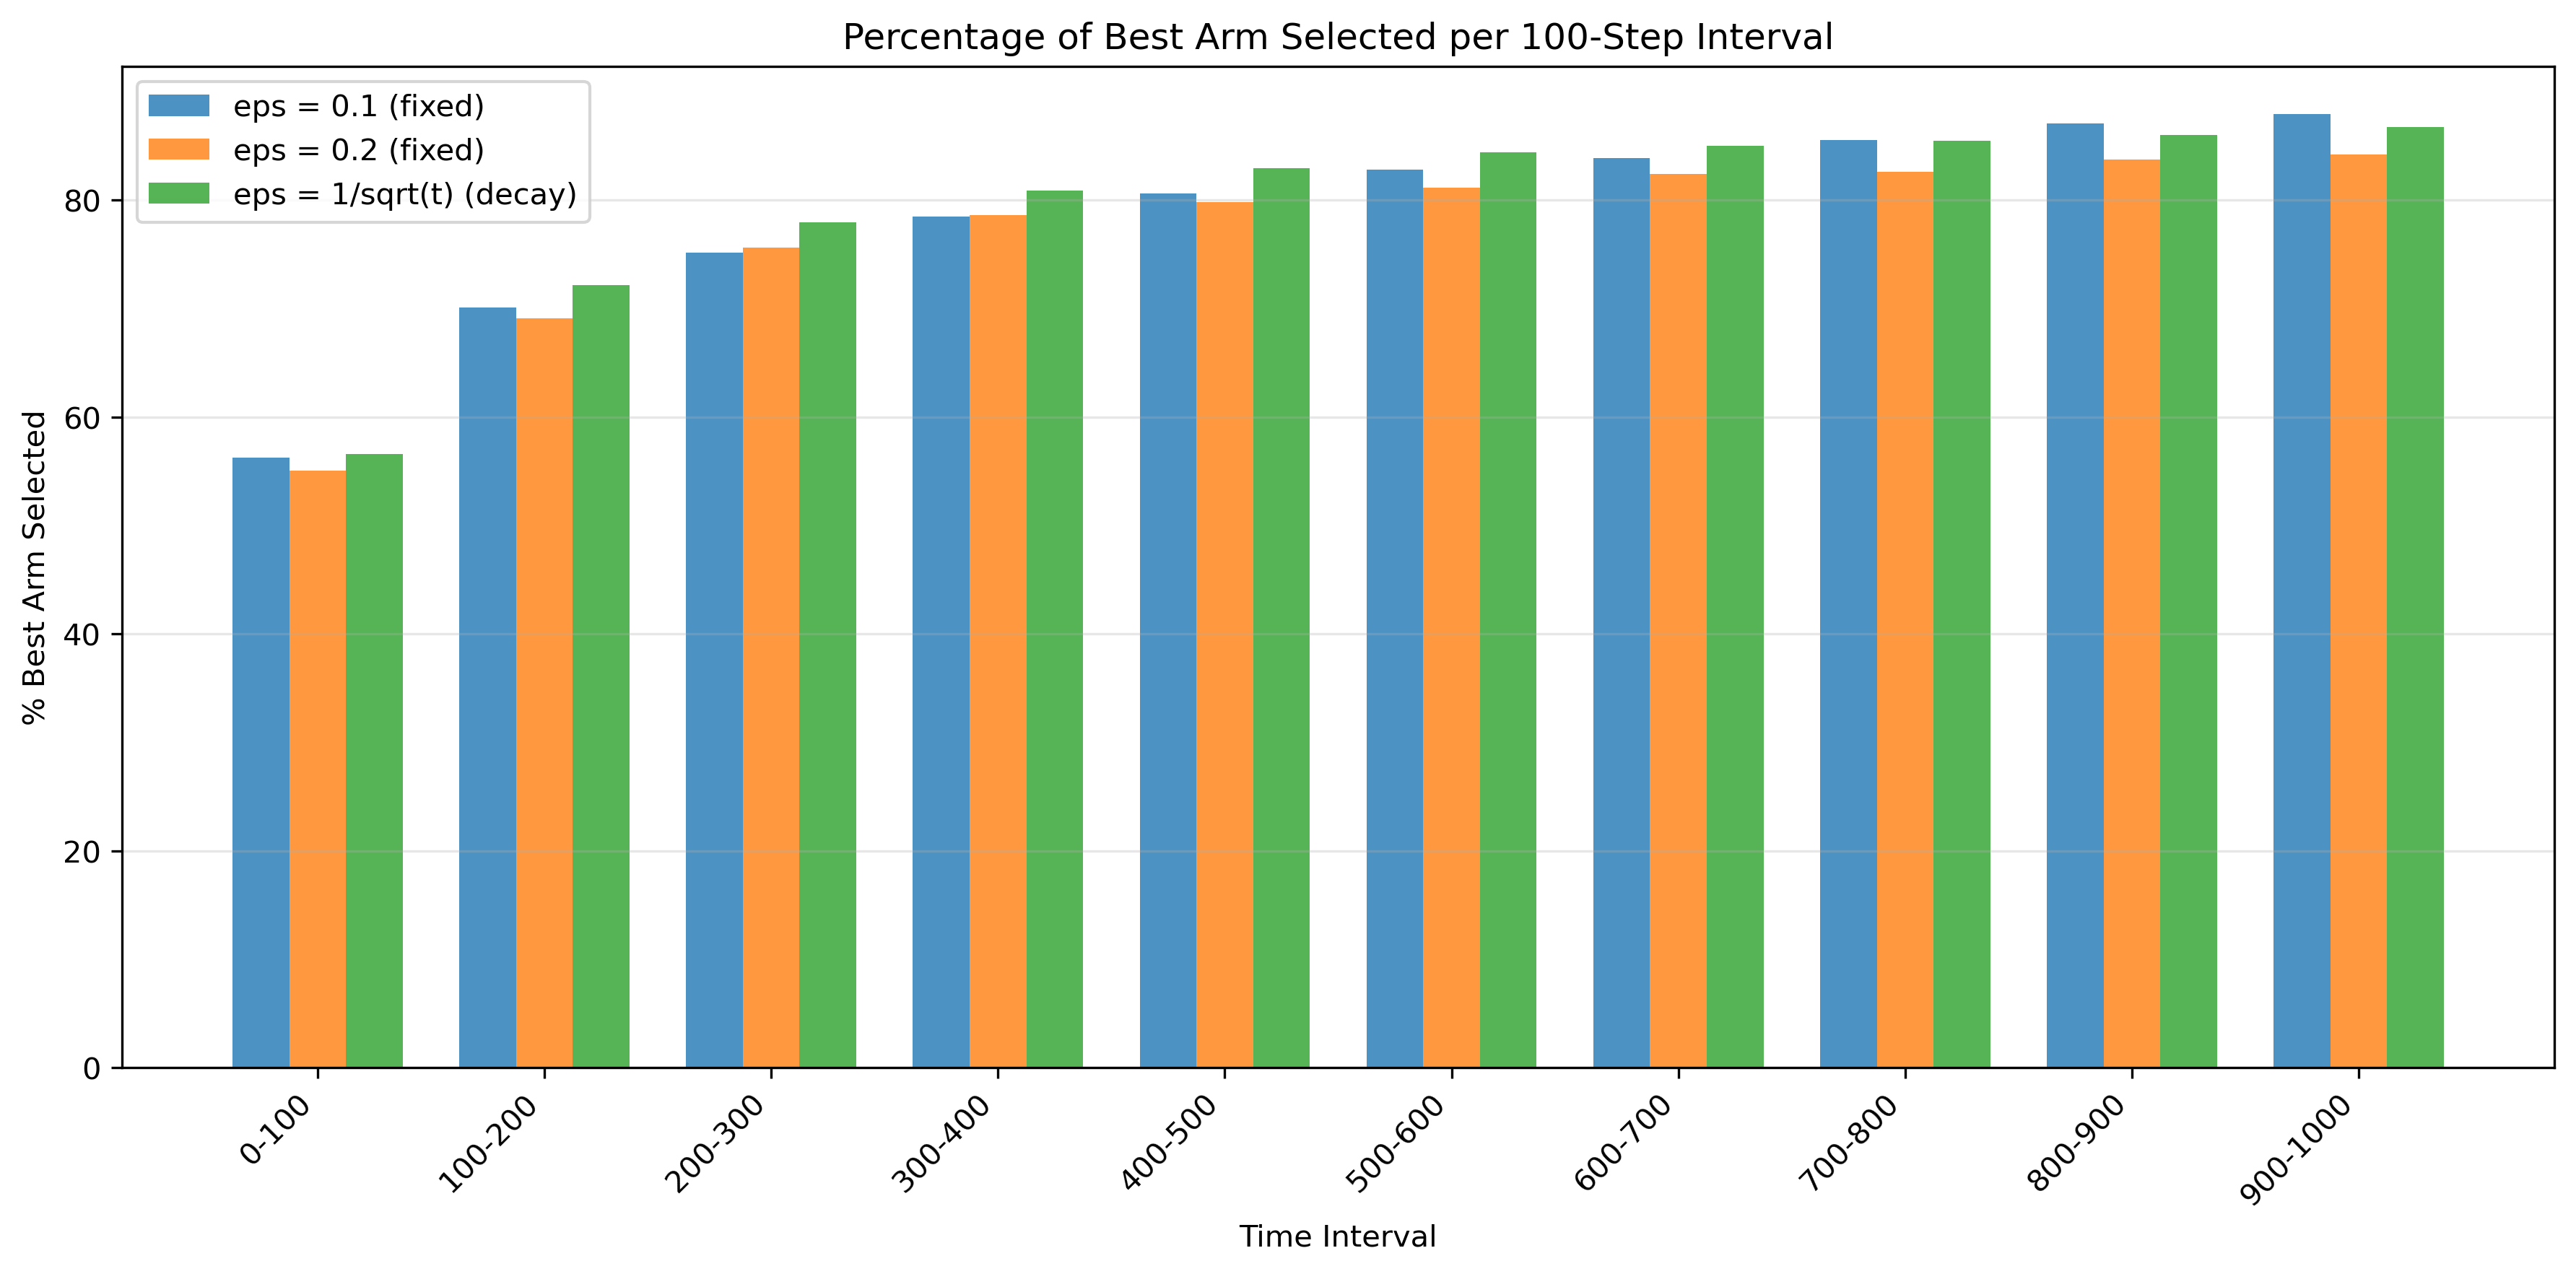
\includegraphics[width=0.75\textwidth]{figures/best_arm_fraction.png}
    \caption{Percentage of best arm selected in intervals of 100 steps}
    \label{fig:best_arm}
\end{figure}

\subsection*{(ii) Different Epsilon Effects}
A small $\varepsilon$ favors exploitation for faster convergence, while a large $\varepsilon$ favors exploration. Decaying $\varepsilon$ optimally shifts from early exploration to late exploitation, achieving no-regret learning ($\lim_{T\to\infty} R(T)/T = 0$).

\subsection*{(iii) Effect of More Arms}
If there were more than three arms, we would expect the best arm to be selected less frequently and convergence to take longer. This is because with $K$ arms, the theoretical upper bound on best arm selection is $1 - \varepsilon + \varepsilon/K$ (the probability of exploit is $1-\epsilon$, then when explore, we still have $1/K$ probability of selecting the best arm), which decreases as $K$ increases, and the algorithm requires more exploration rounds to estimate each arm's reward, delaying accurate identification of the best arm.

\subsection*{(iv) Average Cumulative Regret}

The regret at time $T$ measures the cumulative loss from not always selecting the optimal arm:
\[
R(T) = \sum_{t=1}^{T} \left(\mu^* - \mu_{a_t}\right)
\]
where $\mu^* = 0.5$ is the best arm's expected reward and $\mu_{a_t}$ is the expected reward of the arm selected at time $t$.

\begin{figure}[H]
    \centering
    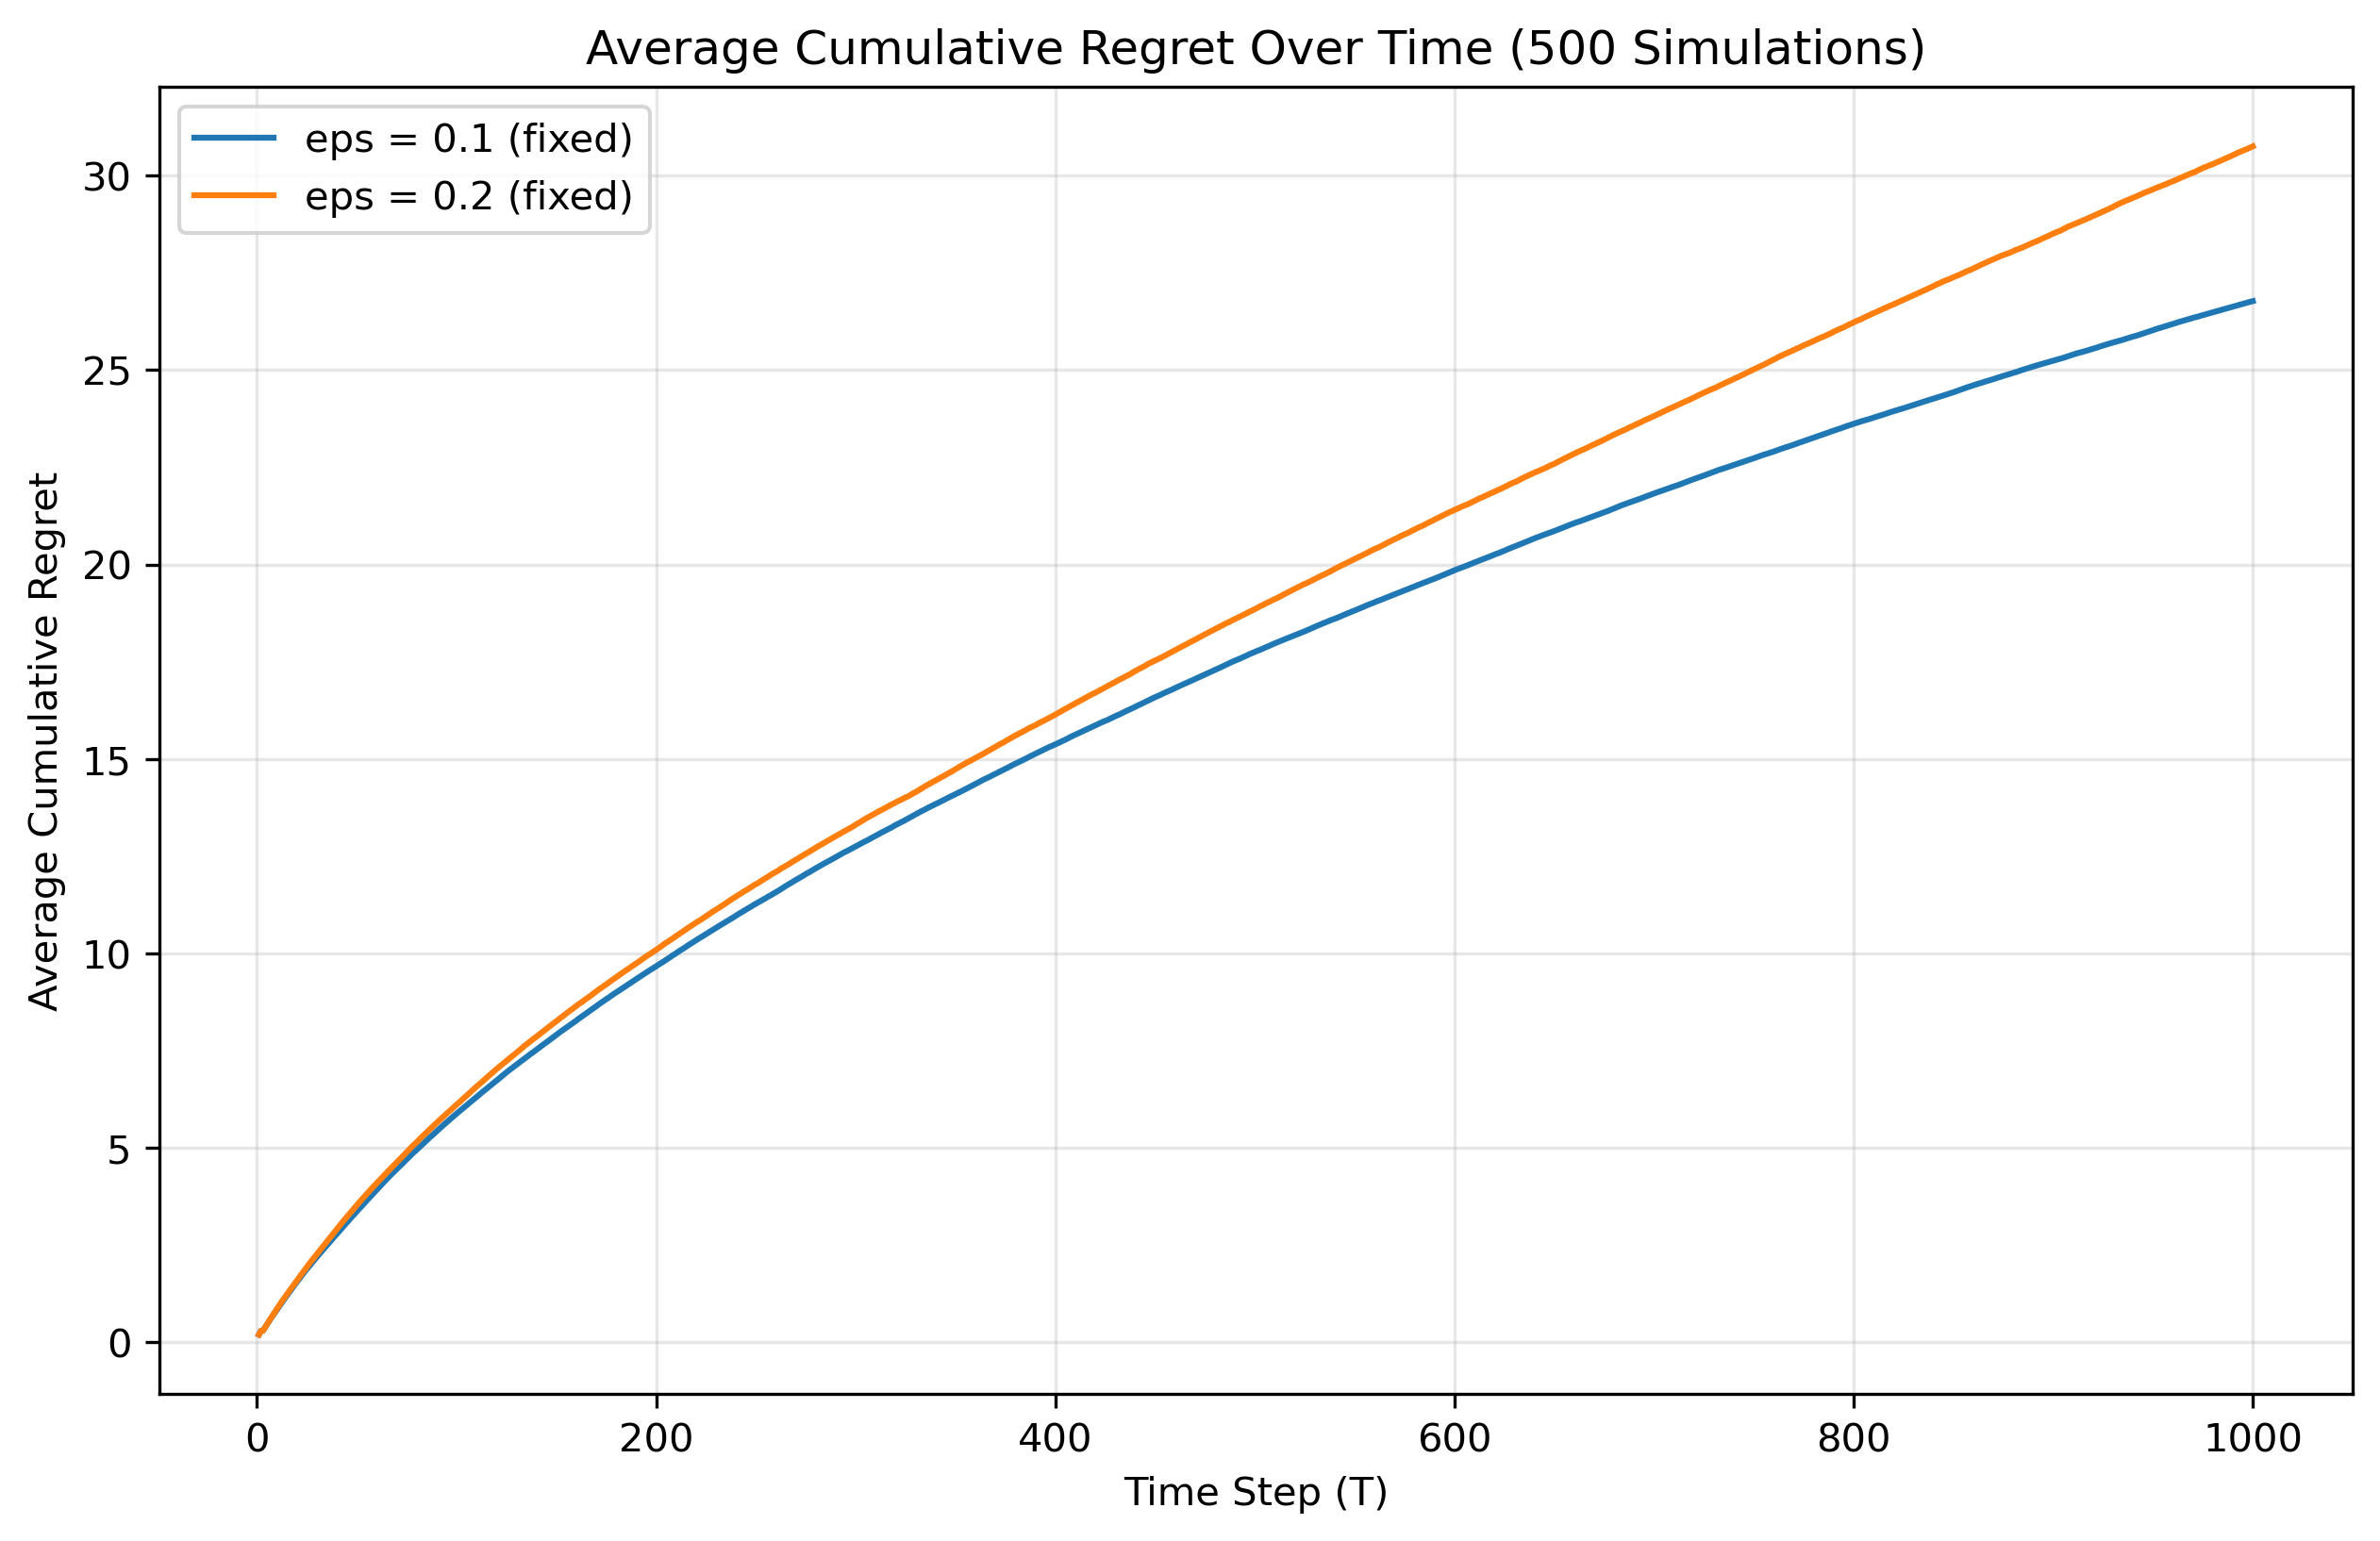
\includegraphics[width=0.6\textwidth]{figures/regret_comparison.png}
    \caption{Average cumulative regret over time for $\varepsilon = 0.1$ and $\varepsilon = 0.2$}
    \label{fig:regret}
\end{figure}

The regret grows linearly in $T$ for both values of $\varepsilon$. This is expected because $\varepsilon$-greedy explores with a fixed probability $\varepsilon$ at every time step, leading to a constant per-step expected regret of $\varepsilon \cdot \bar{\Delta}$, where $\bar{\Delta}$ is the average sub-optimality gap. Higher $\varepsilon$ (0.2) leads to higher regret because the algorithm explores more often, incurring more sub-optimal selections (when the underlying reward doesn't change). After $T = 1000$: $\varepsilon = 0.1$ yields average regret $\approx 27.0$, while $\varepsilon = 0.2$ yields $\approx 31.5$.

\vspace{0.5em}
\noindent\textbf{Conclusion Exercise 1:} It is worth mentioning that while the $\varepsilon$-greedy algorithm is simple and computationally efficient, the choice of $\varepsilon$ represents a direct trade-off between adaptability (flexibility) and efficiency (time to converge). A small $\varepsilon$ converges quickly in a static environment but struggles to adapt if the underlying reward probabilities change over time. Conversely, a larger $\varepsilon$ constantly monitors alternative arms, allowing it to "catch up" faster if the environment shifts, but at the cost of higher steady-state regret.


\newpage
\section*{Exercise 2: Exp3 Algorithm}
%% ════════════════════════════════════════════════════════════

The probability equation:
\[
P_i(t) = (1-\gamma)\frac{W_i(t)}{\sum_j W_j(t)} + \frac{\gamma}{|A|}
\]

\subsection*{(i) How Exp3 Balances Exploration and Exploitation}

Exp3 balances exploration and exploitation by mixing a weighted probability distribution via Weights ($1-\gamma$) and a uniform distribution via Exploration ($\gamma$), while using importance-weighting to ensure rarely-chosen arms still receive fair credit.

\subsection*{(ii) Exploration Comparison: Exp3 vs Epsilon-Greedy}

When $\gamma = \varepsilon$, Exp3 explores more than Epsilon-Greedy. Epsilon-Greedy 'exploits' with $(1-\varepsilon)$ probability to choose only the single best arm 100 percent of the time, whereas Exp3 'exploits' with $(1-\gamma)$ probability using a weighted distribution across all arms. By distributing its exploitation on suboptimal arms, Exp3 inherently maintains a higher level of exploration.

\subsection*{(iii) Area of application of Exp3}

Exp3 is best deployed in dynamic reward environments where the underlying reward distributions change over time (e.g., algorithmic pricing against competitors, or shifting user trends). While Epsilon-Greedy relies on averages reward that are slow to adapt to sudden changes, Exp3 maintains a continuous, weighted exploration of all arms and updates its probabilities exponentially. This exponential scaling allows it to adapt to shifting environments dramatically faster.

%% ════════════════════════════════════════════════════════════
\newpage
\section*{Exercise 3: Optimal Fee Design}
%% ════════════════════════════════════════════════════════════

\textit{Note: The complete Python implementation for Exercise 3 is available in Appendix~\ref{sec:ex3-code}.}
\subsection*{(i) Two Approaches to Choose $b$}

\subsubsection*{Approach 1: A/B Testing (More like Switchback Experiments)}

Run controlled experiments where buyer fee splits $b$ are tested on all users, but we apply them sequentially and randomly on daily/weekly basis, and we put also no treatment period between phases to remove the carryover effects. measuring the resulting platform revenue.

\textbf{Advantage:} Directly measures causal effect of $b$ on revenue without needing to model buyer and seller behavior (model-free), giving reliable real-world estimates.

\textbf{Disadvantage:} Requires exposing users to potentially suboptimal fee splits during the experiment, which incurs opportunity cost and may take significant time to reach statistical significance across all candidate values of $b$.

\subsubsection*{Approach 2: Multi-Armed Bandit (MAB)}

Treat each candidate value of $b$ as an arm and use a bandit algorithm (e.g., Thompson Sampling or UCB) to dynamically learn the best fee split while minimizing regret during the learning process.

\textbf{Advantage:} Learns the optimal $b$ while minimizing cumulative revenue loss during exploration (unlike A/B testing which equally allocates traffic to all arms), adapting quickly as data accumulates.

\textbf{Disadvantage:} Standard MAB assumes stationary rewards, but changing $b$ affects seller pricing strategies (sellers use adaptive algorithms like Exp3), violating the stationarity assumption and potentially leading the MAB to converge to a suboptimal $b$.

\subsection*{(ii) Simulation Results}

The simulation result is shown in Figure~\ref{fig:fee_optimization} and Table~\ref{table:fee_results}.

\begin{figure}[H]
    \centering
    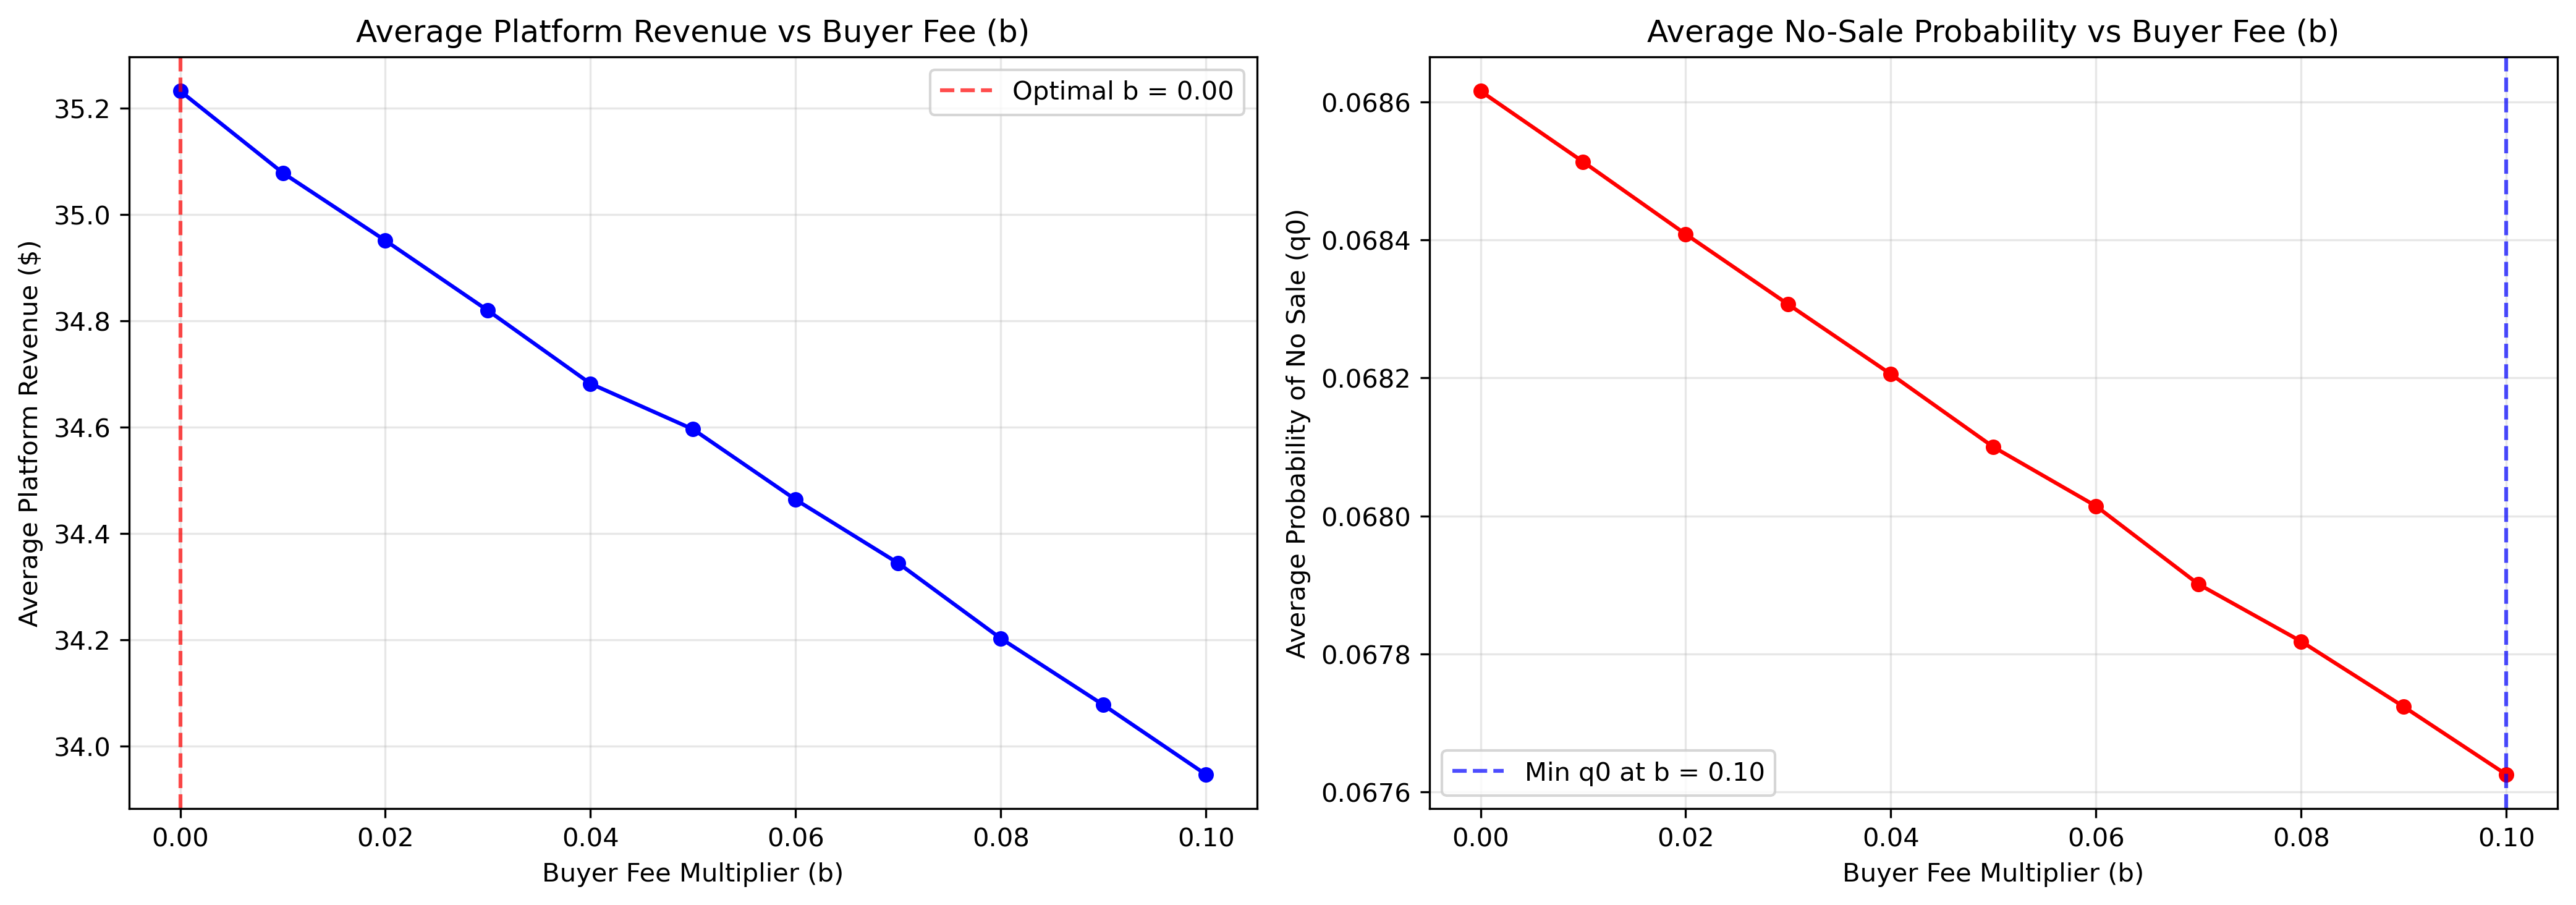
\includegraphics[width=0.80\textwidth]{figures/fee_optimization.png}
    \caption{Average platform revenue and probability of no sale ($q_0$) as a function of $b$}
    \label{fig:fee_optimization}
\end{figure}

\begin{table}[H]
\centering
\small
\begin{tabular}{|c|c|c|}
\hline
\textbf{Buyer Fee (b)} & \textbf{Avg Revenue (\$)} & \textbf{Avg $q_0$} \\
\hline
0.00 & 35.23 & 0.0686 \\
0.01 & 35.08 & 0.0685 \\
0.02 & 34.95 & 0.0684 \\
0.03 & 34.82 & 0.0683 \\
0.04 & 34.68 & 0.0682 \\
0.05 & 34.60 & 0.0681 \\
0.06 & 34.46 & 0.0680 \\
0.07 & 34.34 & 0.0679 \\
0.08 & 34.20 & 0.0678 \\
0.09 & 34.08 & 0.0677 \\
0.10 & 33.95 & 0.0676 \\
\hline
\end{tabular}
\caption{Simulation results for optimal fee design}
\label{table:fee_results}
\end{table}

The value of $b$ that maximizes platform revenue is $b^* = 0.00$ (\$35.23), and the value that minimizes $q_0$ is $b_{\min} = 0.10$ ($q_0 = 0.0676$). 

Interestingly, as the fee burden shifts toward buyers (higher $b$), platform revenue drops, but market activity actually increases (the probability of no sale $q_0$ drops to $0.0676$ at $b=0.10$). This occurs because the Exp3-driven sellers aggressively lower their base prices to compensate for the higher buyer fees. Since the platform's revenue is a fixed 10\% cut of the base price, the sellers' price reductions cause the platform's total revenue to drop, despite the slight increase in sales volume.

\subsection*{(iii) Importance of Minimizing $q_0$}

Minimizing the probability of no sale ($q_0$) is crucial because losing buyers to ``no sale'' events damages long-term platform health by lowering buyer retention, weakening network effects for sellers, and eroding user trust.

\subsection*{(iv) Economic Intuition for Maximizing Revenues}

The economic intuition for maximizing platform revenue is to set $b=0.00$ (placing all fees on sellers), because the platform takes a fixed 10\% cut of the seller's base price $P$. Since buyers make purchasing decisions based on the total effective price $P(1+b)$, shifting the fee $b$ to buyers forces sellers to lower their base price $P$ to attract buyers, which mathematically shrinks the platform's revenue cut.

\subsection*{(v) Disadvantages of Standard MAB for Learning $b$}

\begin{enumerate}
    \item \textbf{Non-stationarity:} Sellers will adapt their pricing strategies (unknown pattern) to react to changes in $b$, so the reward distribution for each arm (each value of $b$) is non-stationary, violating the MAB assumption that each arm has a fixed reward distribution.
    \item \textbf{Competitive Settings:} Algorithms like UCB or TS perform poorly when rewards depend on the actions of strategic competitors, when the platform changes $b$, the competing sellers react by adjusting their pricing strategies, when we don't know their strategies, it will be hard to predict the dynamics and to reliably learn the optimal $b$.
\end{enumerate}

\subsection*{(vi) Switchback Experiment Design}

To choose the two fees to test, we should select $b=0.00$ and $b=0.10$ which ensures the values are sufficiently different to detect a meaningful statistical effect. The key limitation is that seller pricing algorithms (Exp3) carry over state between periods, creating \textbf{carryover effects} that bias the treatment effect estimate.

%% ════════════════════════════════════════════════════════════
\newpage
\section*{Exercise 4: DoorDash Messaging Optimization}
%% ════════════════════════════════════════════════════════════

\textit{Note: The complete Python implementation for Exercise 4 is available in Appendix~\ref{sec:ex4-code}.}

\subsection*{(i) DoorDash's Choice of Thompson Sampling}

DoorDash chose MAB with TS over other bandit algorithms because it naturally handles the exploration-exploitation trade-off through posterior sampling, which is computationally efficient for large-scale systems, and it performs well empirically with binary outcomes (accept/reject). 

They preferred it over offline ML methods because TS can \textbf{learn and adapt in real-time} without a separate training phase, handles the cold-start problem for new Dashers through informative priors, and avoids the feedback loop issues of offline models that are trained on non-representative historical data. 

They tested the algorithm using \textbf{switchback experiments} (alternating between TS and random/baseline messaging in different time periods) to measure the causal impact on Dasher conversion rates and supply availability.

\subsection*{(ii) Switchback Experiment Simulation}

The simulation result shows that Thompson Sampling achieves a significantly higher conversion rate (72.50\%) compared to random messaging (49.78\%), with a highly significant ATE of 0.2272. Figure~\ref{fig:switchback} and Table~\ref{table:switchback_results} summarize the simulation results.

\begin{figure}[H]
    \centering
    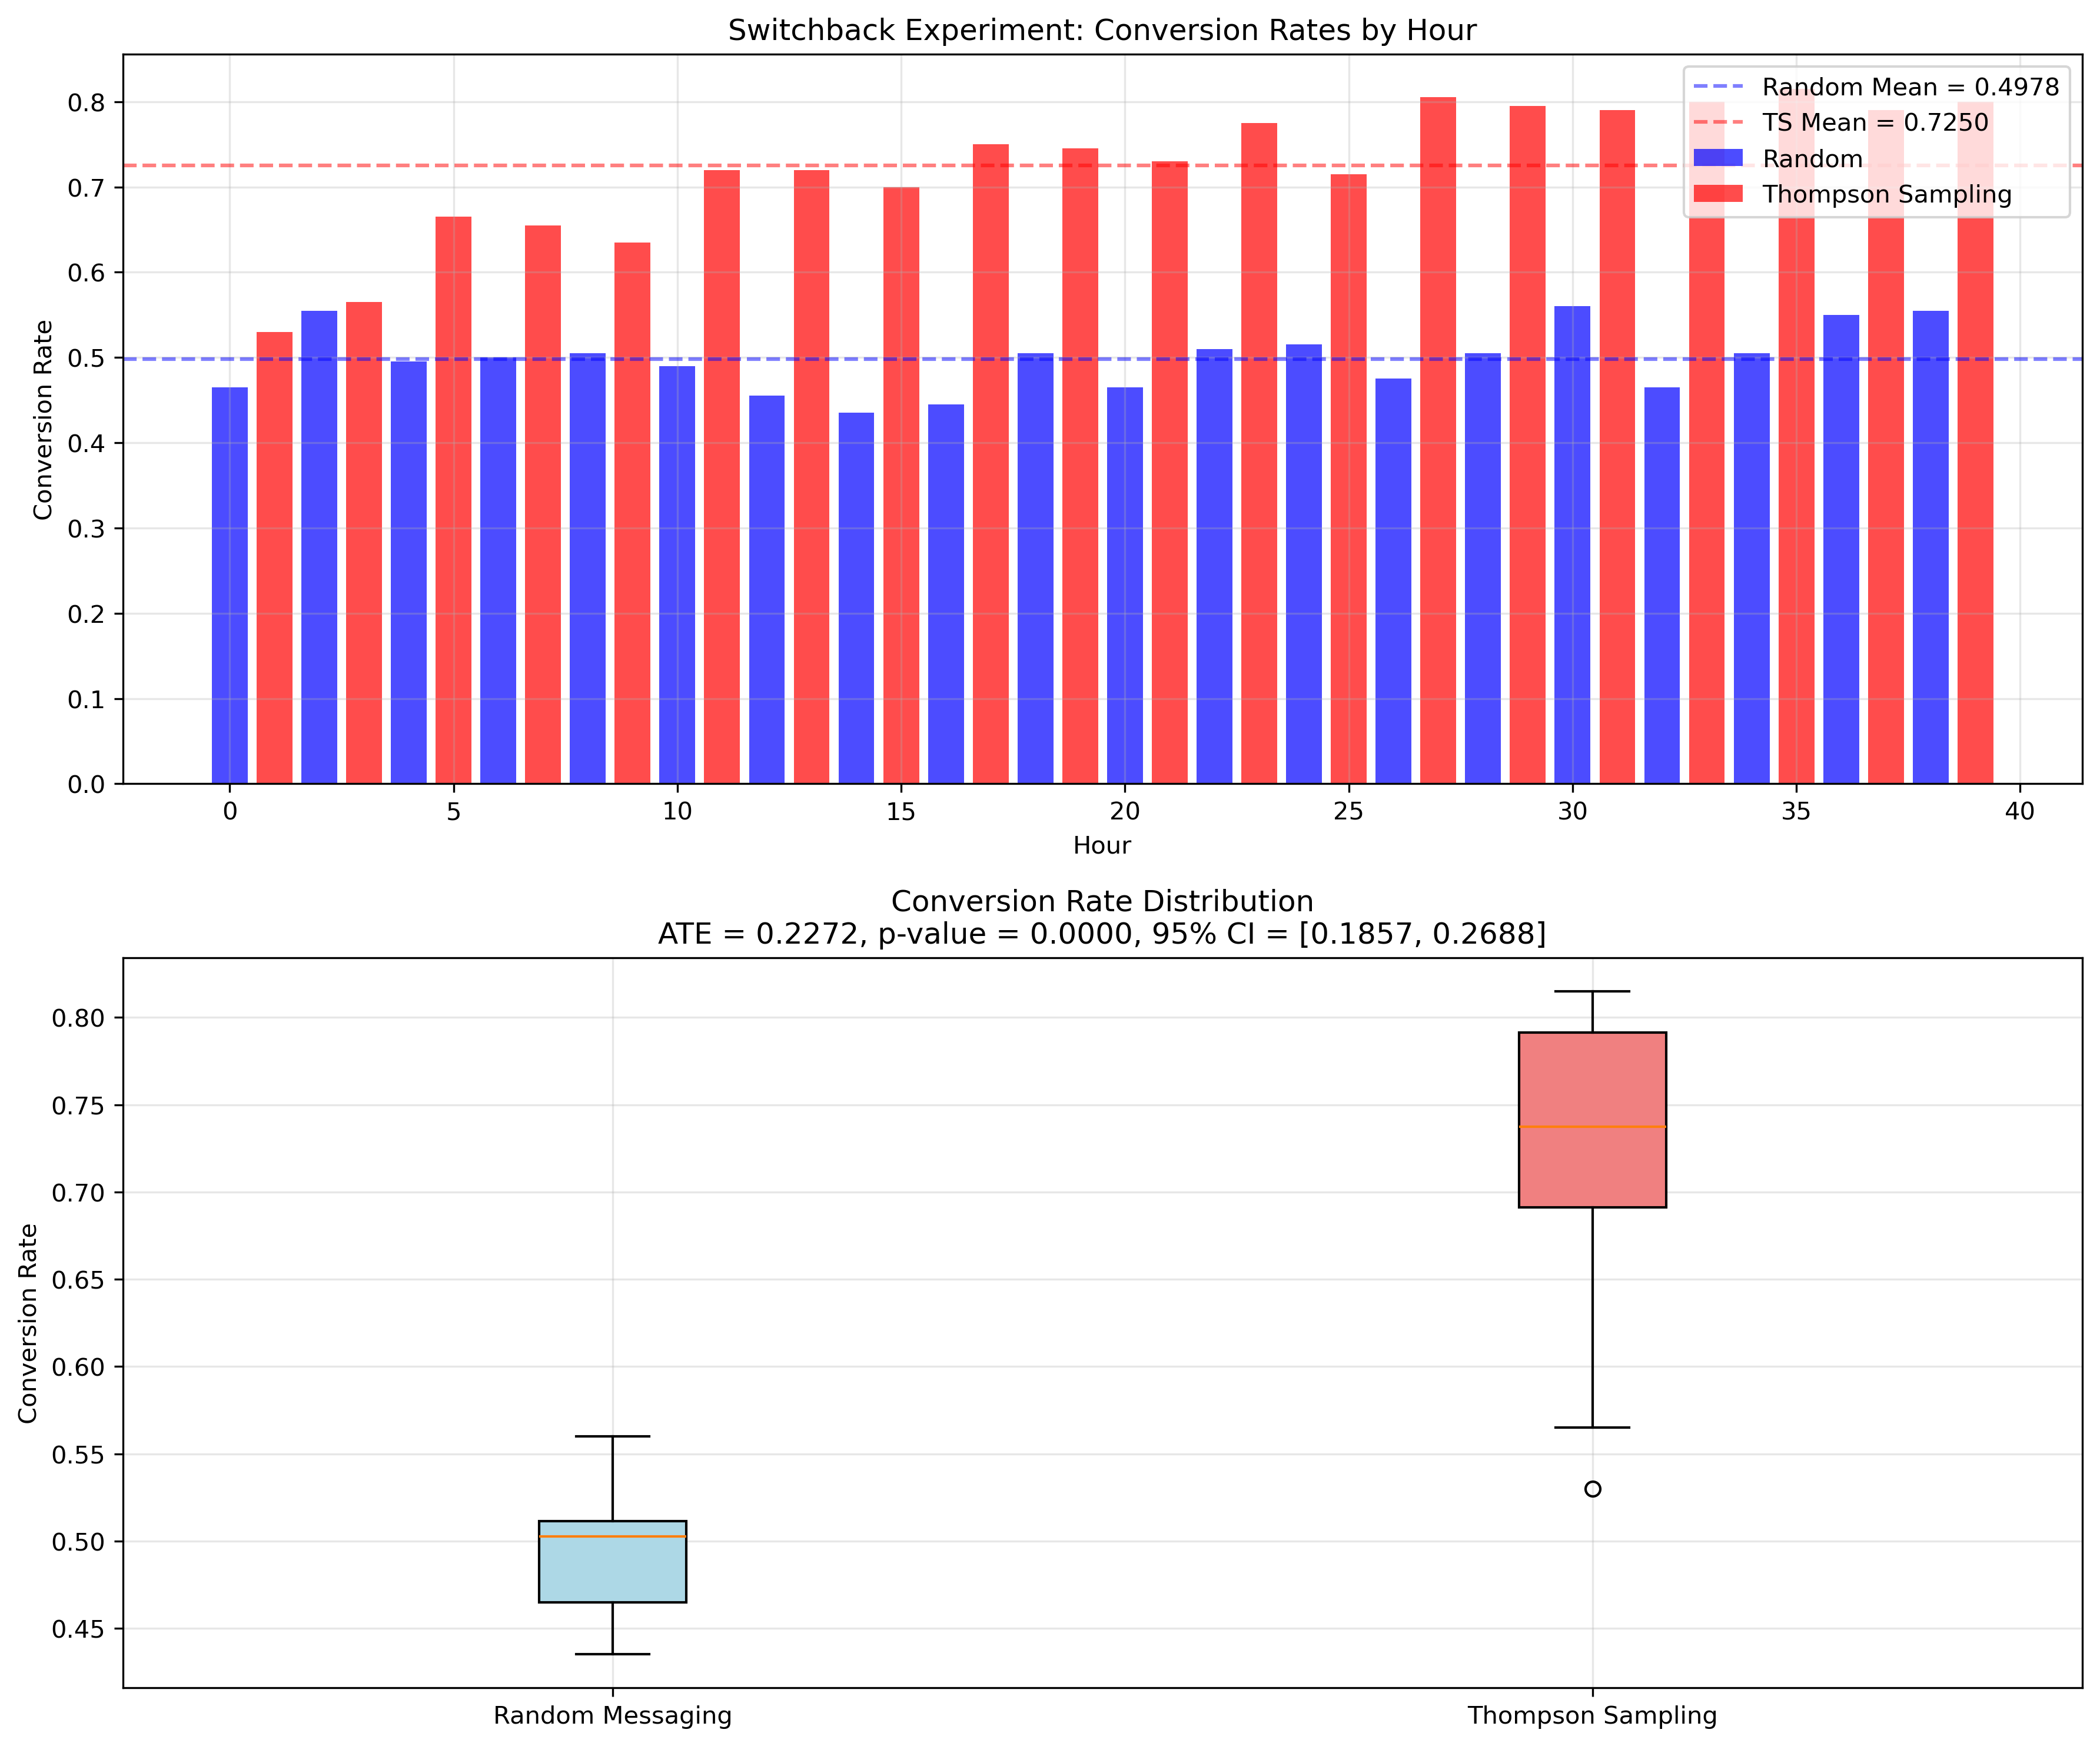
\includegraphics[width=0.7\textwidth]{figures/switchback_experiment.png}
    \caption{Switchback experiment results: hourly conversion rates and distribution comparison}
    \label{fig:switchback}
\end{figure}

\begin{table}[H]
\centering
\small
\begin{tabular}{|l|c|}
\hline
\textbf{Metric} & \textbf{Value} \\
\hline
Mean Random Conversion Rate & 0.4978 \\
Mean TS Conversion Rate & 0.7250 \\
Average Treatment Effect (ATE) & 0.2272 \\
p-value & $< 0.0001$ \\
95\% Confidence Interval & [0.1857, 0.2688] \\
\hline
\end{tabular}
\caption{Switchback experiment analysis results}
\label{table:switchback_results}
\end{table}

\subsection*{(iii) Why the ATE is Misleading}

The ATE from this switchback experiment is misleading because it \textbf{overestimates} the true treatment effect due to a violation of SUTVA. Specifically, the experiment suffers from strong \textbf{carryover effects} (or spillover). Because the same population of Dashers is used across alternating hours, messaging a Dasher in one hour directly impacts their availability and likelihood to accept a delivery in the next hour. Therefore, the outcomes observed during the control (Random) periods are heavily contaminated by the actions taken during the preceding treatment (Thompson Sampling) periods, violating the assumption of no interference.

\subsection*{(iv) Possible Solution}

To mitigate these carryover effects, we should introduce washout periods between the control and treatment phases. By adding a sufficient time buffer where we exclude data from our analysis immediately after an algorithm switch, we allow the Dashers' states to reset.
%% ════════════════════════════════════════════════════════════
\newpage
\appendix
\section{Exercise 1 Complete Code}
\label{sec:ex1-code}

Below is the complete Python code for Exercise 1, which implements the $\varepsilon$-greedy multi-armed bandit algorithm.

\lstinputlisting[caption={exercise1.py -- Complete Implementation}, language=Python]{exercise1.py}

\section{Exercise 3 Complete Code}
\label{sec:ex3-code}
Below is the complete Python code for Exercise 3, which simulates the optimal fee design with Exp3 sellers and multinomial logit demand.

\lstinputlisting[caption={exercise3.py -- Complete Implementation}, language=Python]{exercise3.py}

\section{Exercise 4 Complete Code}
\label{sec:ex4-code}

Below is the complete Python code for Exercise 4, which implements Thompson Sampling messaging and the switchback experiment.

\lstinputlisting[caption={exercise4.py -- Complete Implementation}, language=Python]{exercise4.py}

\end{document}
